\chapter{Выполнение задания}

В этой части будет представлен код алгоритма, а также графовые представления для него.

\section{Код программы}

В листинге \ref{lst:alg} представлен код программы на языке $Python~\cite{python-lang}$, которая разделяет текст на токены и выводит их на экран в формате: \textit{Token: [текст токена] | Lemma: [лемма токена] | POS: [часть речи токена]}.


\begin{center}
	\captionsetup{justification=raggedright,singlelinecheck=off}
	\begin{lstlisting}[label=lst:alg,caption=код программы]
import spacy
import pymorphy2
nlp = spacy.load('ru_core_news_sm')
morph = pymorphy2.MorphAnalyzer()
with open('input.txt', 'r') as file:
	text = file.read()                                      #-1
punctuation_marks = ['.', '!', '?']                         #1
sentences = []                                              #2
current_sentence = ''                                       #3
for char in text:                                           #4               
	if char not in punctuation_marks:                       #5      
		current_sentence += char                            #6
	if char in punctuation_marks:                           #7
		current_sentence = current_sentence.strip()         #8
		sentences.append(current_sentence)                  #9
		current_sentence = ''                               #10
if current_sentence.strip() != '':                          #11
	sentences.append(current_sentence.strip())              #12
for sentence in sentences:                                  #13
	doc = nlp(sentence)                                     #14
	for token in doc:                                       #15
		analyzed_token = morph.parse(token.text)[0]         #16
		print(f'Token: {token.text}\t| Lemma: {analyzed_token.normal_form}\t| POS: {analyzed_token.tag.POS}')
	\end{lstlisting}
\end{center}


\section{Графовые представления}

Далее предствлены рисунки со следующими графовыми моделями алгоритма:
\begin{enumerate}[label=\arabic*)]
	\item \ref{fig:oper_graph} --- граф управления;
	\item \ref{fig:inf_graph} --- информационый граф;
	\item \ref{fig:oper_his} --- граф операционной истории;
	\item \ref{fig:inf_his} --- граф информационой истории.
\end{enumerate}

\begin{figure}[h!]
	\centering
	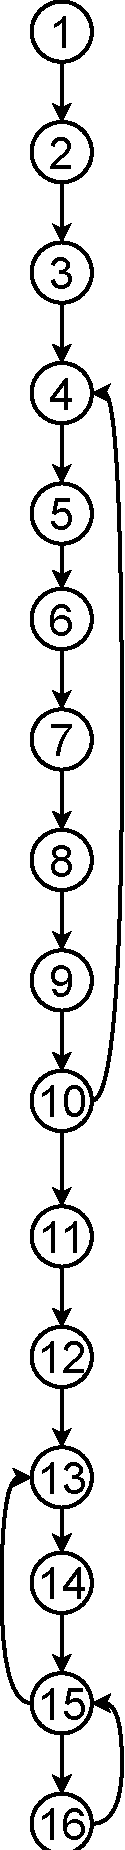
\includegraphics[width=0.1\linewidth]{img/gu}
	\caption{граф управления}
	\label{fig:oper_graph}
\end{figure}

\begin{figure}[h!]
	\centering
	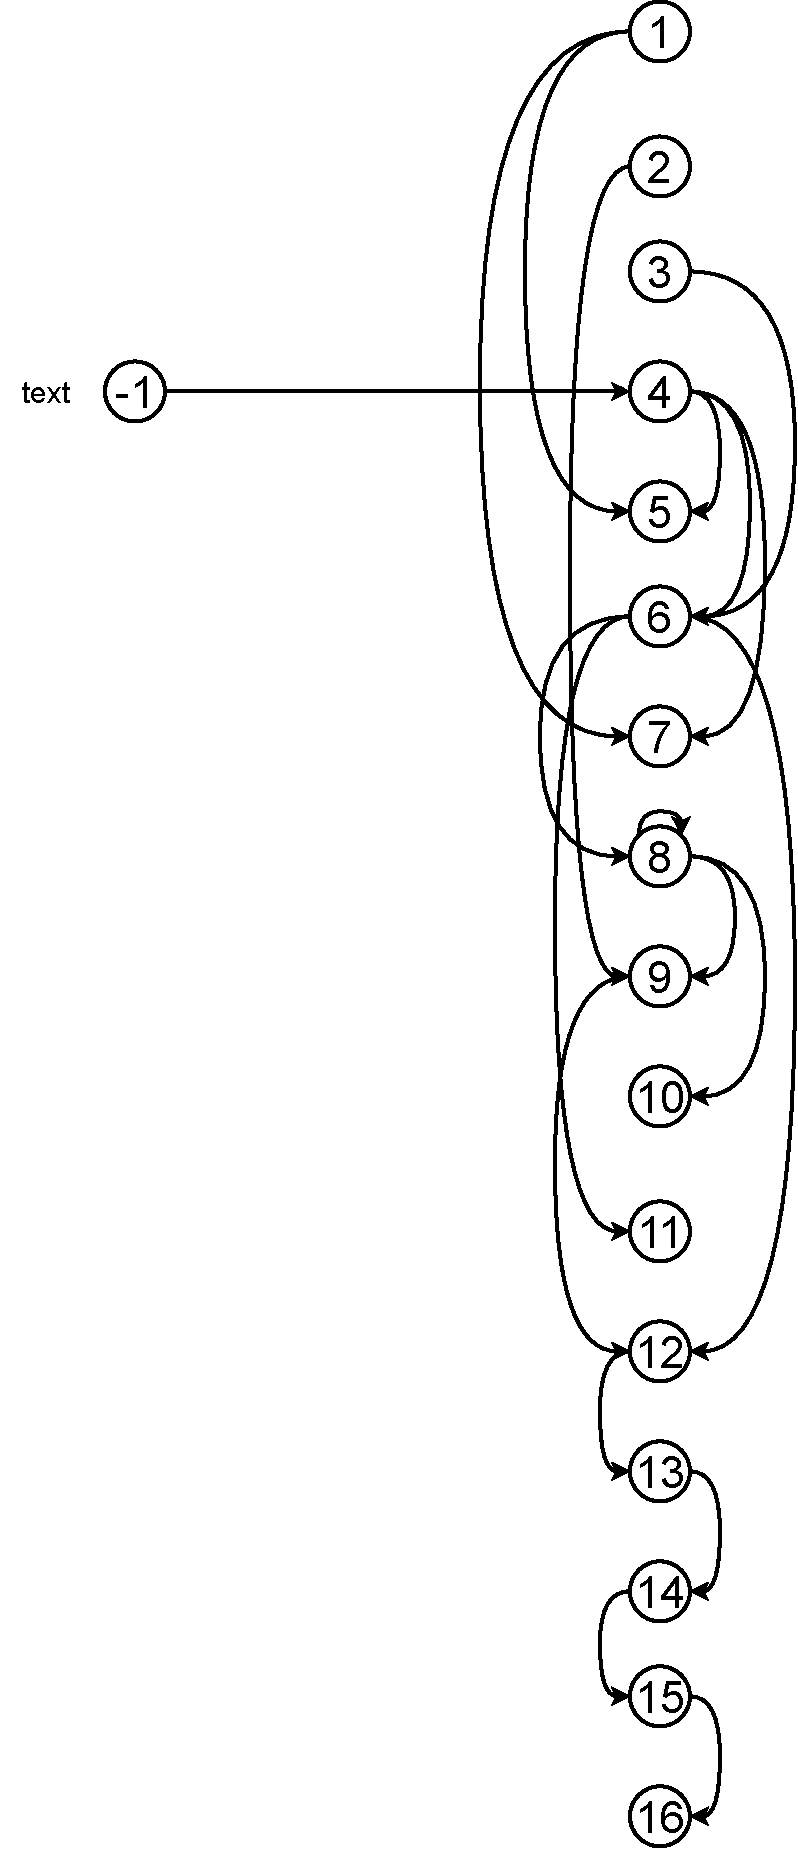
\includegraphics[width=0.6\linewidth]{img/ig}
	\caption{информационый граф}
	\label{fig:inf_graph}
\end{figure}

\begin{figure}[h!]
	\centering
	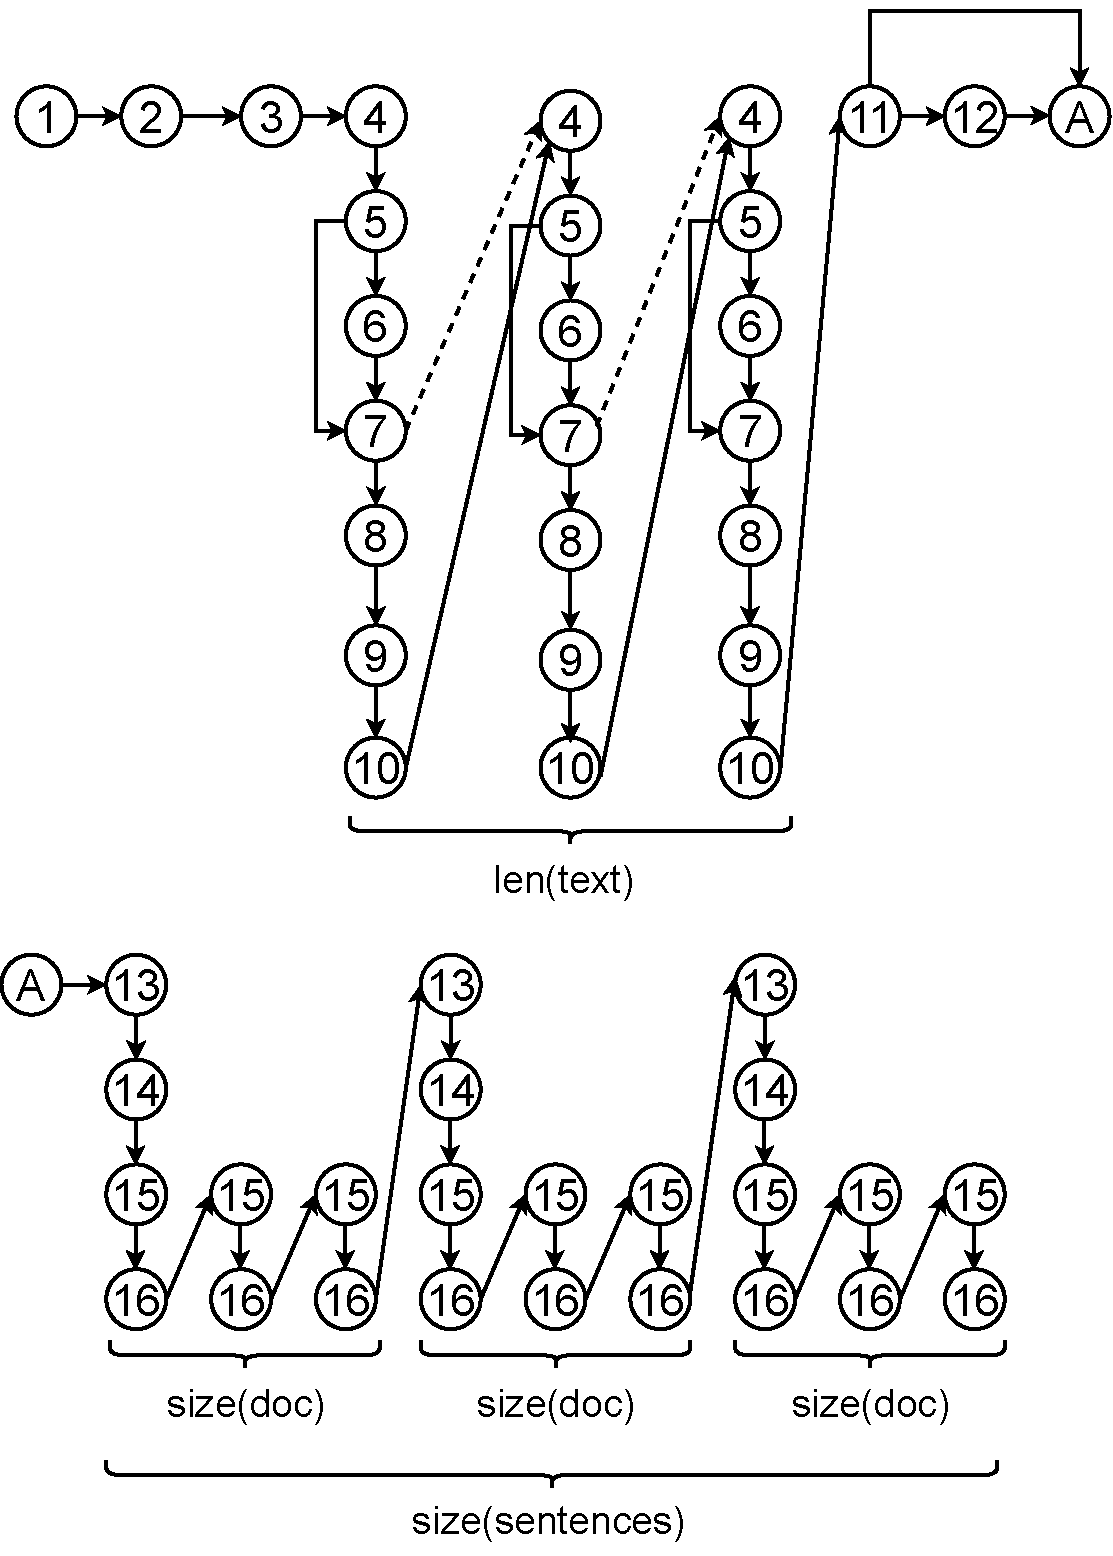
\includegraphics[width=0.9\linewidth]{img/oi}
	\caption{граф операционной истории}
	\label{fig:oper_his}
\end{figure}

\begin{figure}[h!]
	\centering
	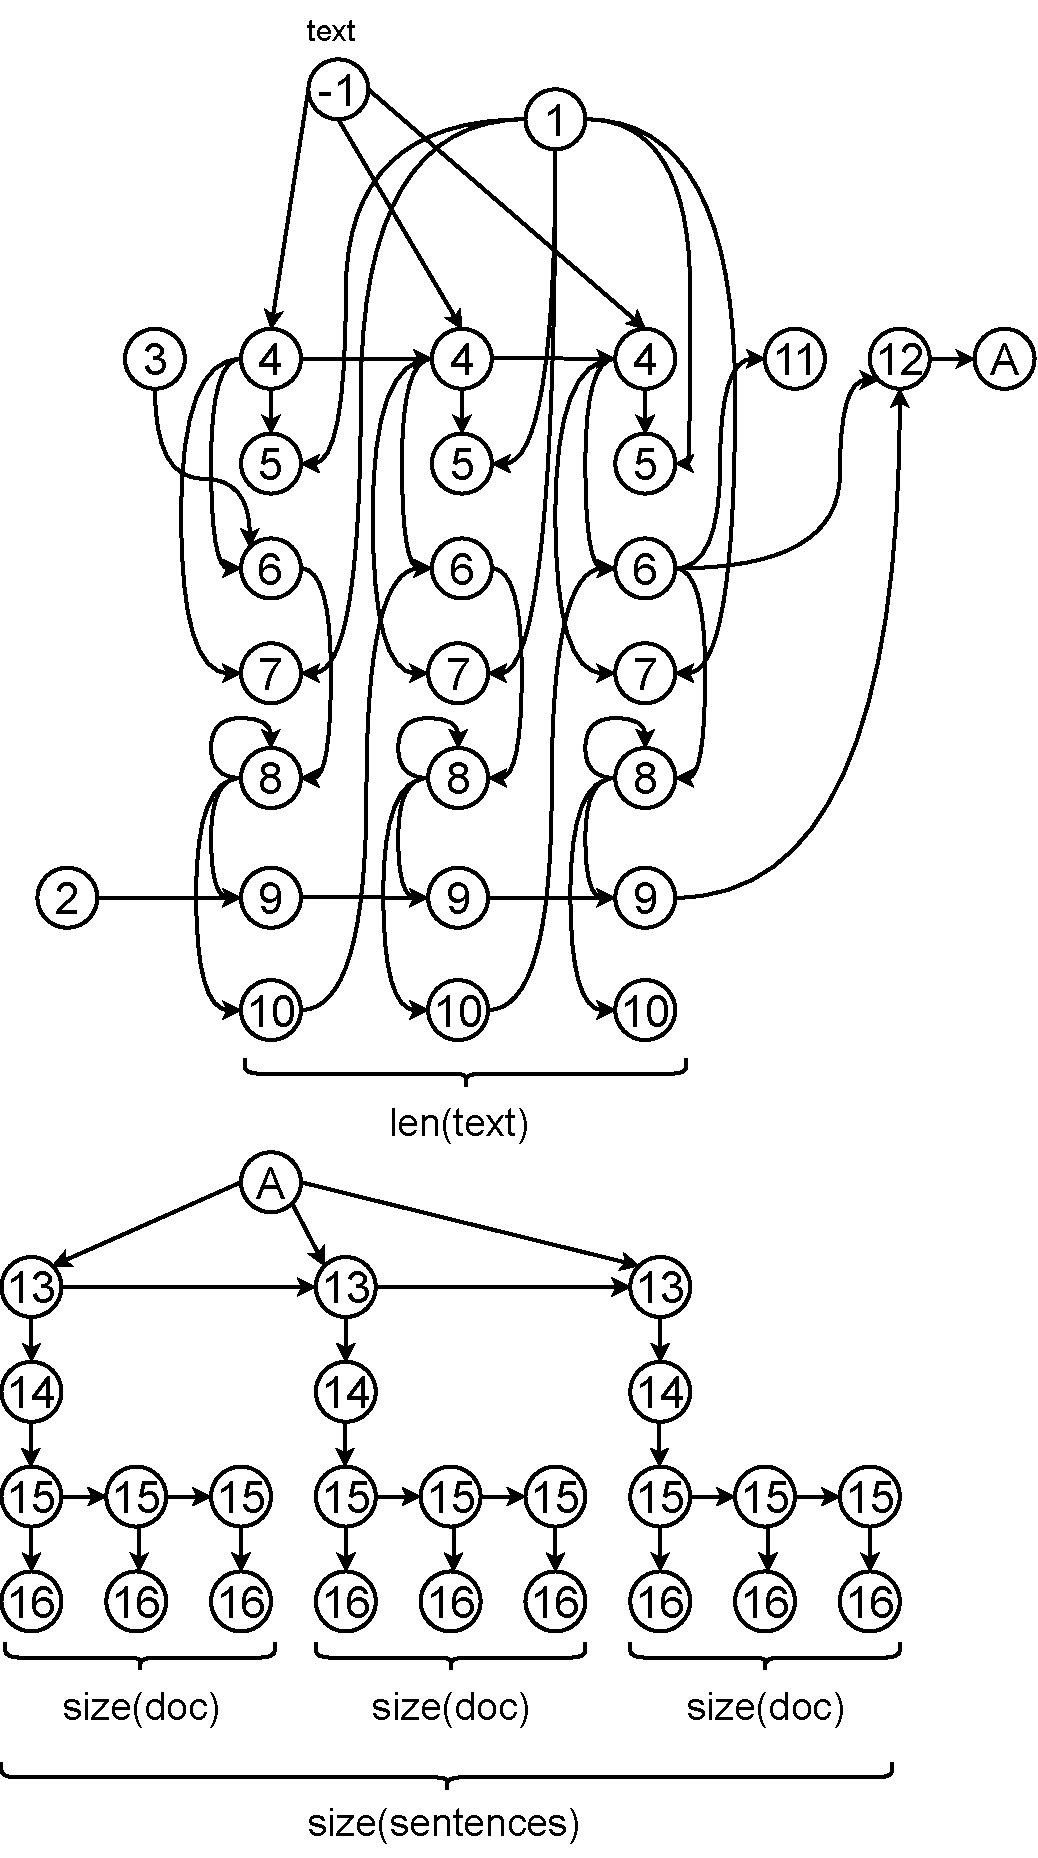
\includegraphics[width=0.8\linewidth]{img/ii}
	\caption{граф информационой истории}
	\label{fig:inf_his}
\end{figure}
\clearpage

\section*{Вывод}

Программа разделяет текст на независимые предложения, а затем обрабатывает их.
Можно разделить обработку предложений на несколько отдельных потоков.